\item \textbf{Finally, repeat the analysis in 3 but for a VAR-based approach. Explore the relationships between the chosen variables using appropriate tools. Again, there is no fixed number of variables assigned – use your judgement and justify your decisions.  Using a VAR framework, show the impact of including additional variables in your prediction. Repeat the analysis in 2 (a) and (b) using the updated models.} 

\textit{Likewise the last question, we visualized the first nine signals to see what kind of data we have.} 

\begin{figure}[H]
    \centering
    \begin{minipage}[b]{1\textwidth}
        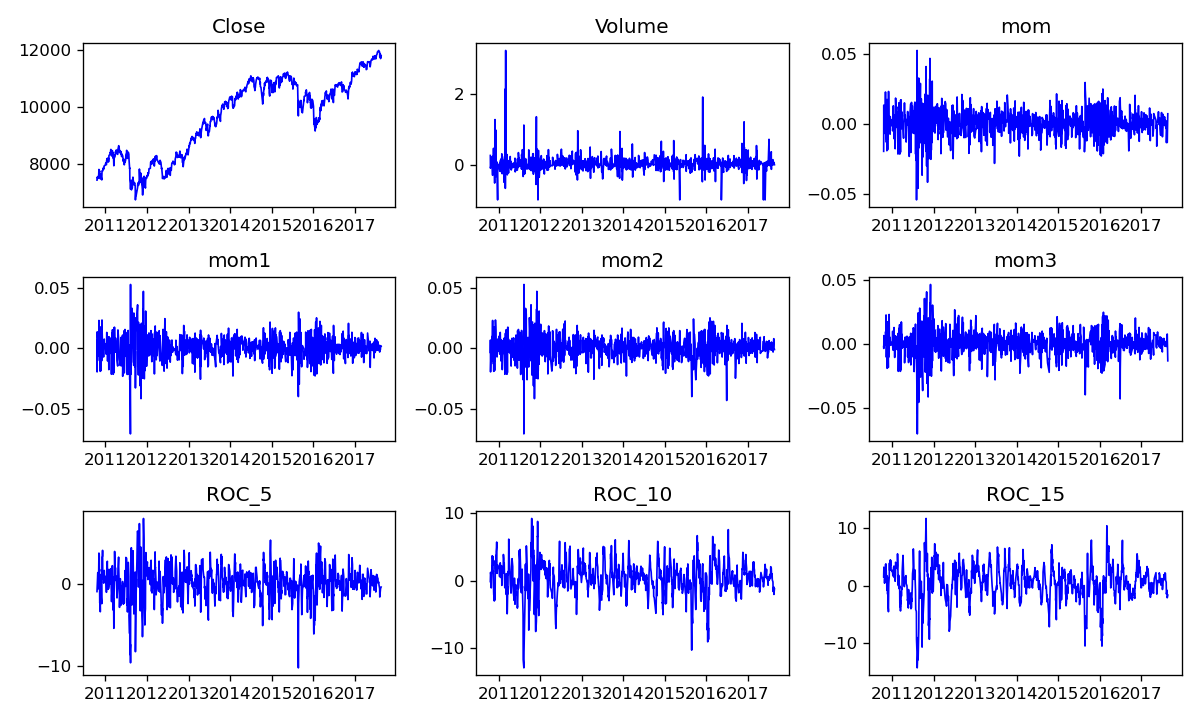
\includegraphics[width=\textwidth]{figures/Ass2/Ass2_Q3_raw_signal.png}
    \end{minipage}
    \caption{The visualization of the first nine columns.}
    \label{fig:Ass2_Q4_raw_signal}
\end{figure}


\textit{Before any transformation, we needed to find out which variables must choose, so that we applied two tools, Granger causality and Johanson's Cointegration test. Granger causality test implemented over the first 20 variables. Then we used the second test on variables that were Granger causes. Tables \ref{tab:Ass2_Q4_Granger_results1} and \ref{tab:Ass2_Q4_coin} show the results of these two tests.
Based on these tests, signals mom, mom1, ROC\_X and EMA\_X had a relation with the target variable ("Close price"). We stored these variables for the next steps.}

\begin{table}[H]
\centering
\caption{The result of Granger causality test.}
\label{tab:Ass2_Q4_Granger_results1}
\begin{tabular}{rlrrc}
\toprule
\# & Variable Name &  min\_p\_value &   lag &  Causality \\
\midrule
1 & Close   &       1.0000 &   1.0 &        - \\
2 & Volume  &       0.2613 &  10.0 &        - \\
3 & mom     &       0.0022 &   8.0 &        \Tik \\
4 & mom1    &       0.0285 &   7.0 &        \Tik \\
5 & mom2    &       0.2049 &   2.0 &        - \\
6 & mom3    &       0.0860 &   1.0 &        - \\
7 & ROC\_5   &       0.0024 &   1.0 &        \Tik \\
8 & ROC\_10  &       0.0036 &   1.0 &        \Tik \\
9 & ROC\_15  &       0.0037 &   1.0 &        \Tik \\
10 & ROC\_20  &       0.0010 &   9.0 &        \Tik \\
11 & EMA\_10  &       0.0021 &   1.0 &        \Tik \\
12 & EMA\_20  &       0.0014 &   1.0 &        \Tik \\
13 & EMA\_50  &       0.0008 &   9.0 &        \Tik \\
14 & EMA\_200 &       0.0035 &   9.0 &        \Tik \\
15 & DTB4WK  &       0.2096 &   1.0 &        - \\
16 & DTB3    &       0.1918 &   1.0 &        - \\
17 & DTB6    &       0.2826 &  10.0 &        - \\
18 & DGS5    &       0.5876 &   5.0 &        - \\
19 & DGS10   &       0.3805 &   5.0 &        - \\
20 & Oil     &       0.0120 &   7.0 &        \Tik \\
\bottomrule
\end{tabular}

\end{table}


\begin{table}[H]
\centering
\caption{The result of Johanson's Cointegration test.}
\label{tab:Ass2_Q4_coin}
\begin{tabular}{rlrrl}
\toprule
\# &  Variable Name &   Test Stat & C(95\%) & Signif \\
\midrule
1 & Close  &  2460.9    & 311.1280 &    True \\
2 & mom    &  1996.6     & 263.2603   & True\\
3 & mom1   &  1666.7     & 219.4051   & True\\
4 & ROC\_5  &  1340.7    & 179.5190 &    True\\
5 & ROC\_10 &  1031.2    & 143.6690 &    True\\
6 & ROC\_15 &  804.2     & 111.7797   & True\\
7 & ROC\_20 &  628.4     & 83.9383    & True\\
8 & EMA\_10 &  459.3     & 60.0627    & True\\
9 & EMA\_20 &  305.6     & 40.1749    & True\\
10 & EMA\_50 &  183.3     & 24.2761    & True\\
11 & EMA\_200 &  81.8     & 12.3212    & True\\
12 & Oil    &  2.7      & 4.1296     & False\\ 
\bottomrule
\end{tabular}

\end{table}


\textit{As figure \ref{fig:Ass2_Q4_raw_signal} shown, signals had a different range. Therefore, we standardized all data to have the same scale. Figure \ref{fig:Ass2_Q4_standard_data} indicates the standardized variables. Also, we applied \gls{ADF} on these signals to find out that these signals were stationary or non-stationary. Table \ref{tab:Ass2_Q4_ADF_results} shows the result of this test on the dataset.}

\begin{figure}[H]
    \centering
    \begin{minipage}[b]{1\textwidth}
        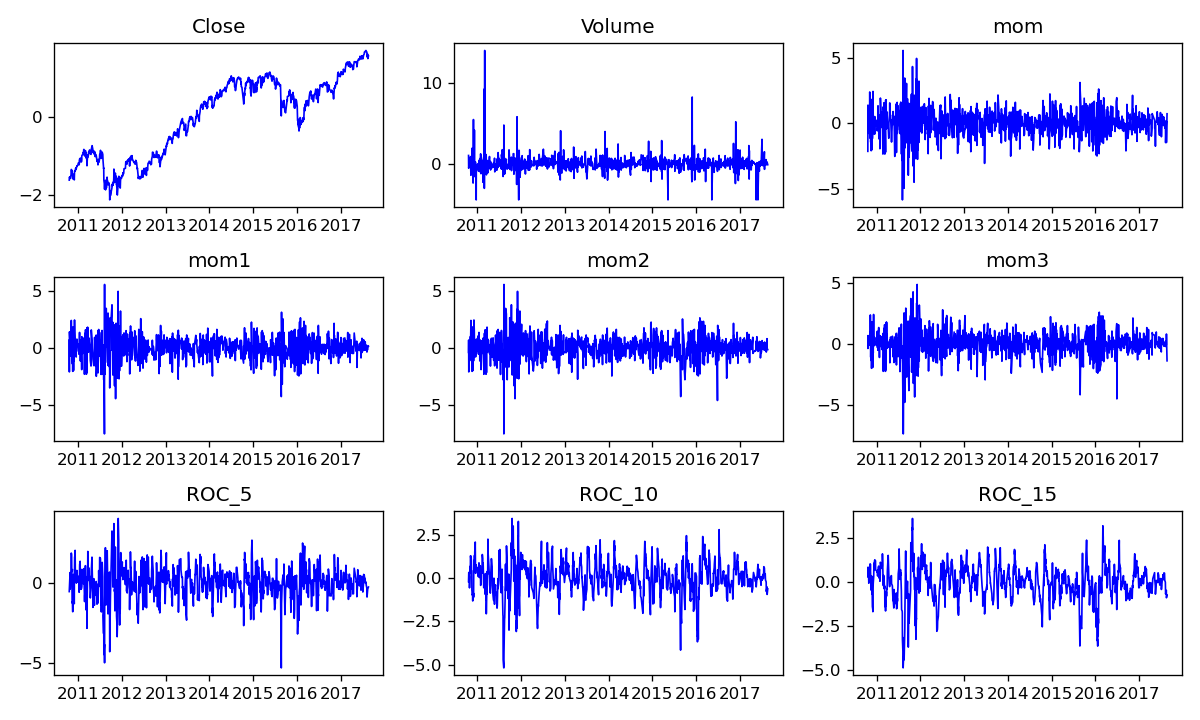
\includegraphics[width=\textwidth]{figures/Ass2/Ass2_Q4_standard_data.png}
    \end{minipage}
    \caption{The visualization of the first nine columns. Columns were standardized.}
    \label{fig:Ass2_Q4_standard_data}
\end{figure}


\begin{table}[H]
\centering
\caption{The result of the \gls{ADF} on the dataset.}
\label{tab:Ass2_Q4_ADF_results}
{\tiny
\hspace*{-2cm}\begin{tabular}{lrrrrrrrrrrrr}
\toprule
{} &        Close &           mom &         mom1 &         ROC\_5 &        ROC\_10 &        ROC\_15 &        ROC\_20 &       EMA\_10 &       EMA\_20 &       EMA\_50 &      EMA\_200 &           Oil \\
\midrule
ADF Statistic               &    -1.085 & -12.134 &   -38.465 & -10.619 & -9.753 & -6.995 & -8.074 &    -0.967 &    -0.882 &    -0.791 &    -0.585 & -8.920 \\
p-value                     &     0.7 &  1.7e-22 &     0 &  5.5e-19 &  7.9e-17 &  7.5e-10 &  1.5e-12 &     0.7 &     0.7 &     0.8 &     0.8 &  1.0e-14 \\
\# Lags Used                  &     2 &  11 &     0 &  9 &  6 &  16 &  5 &     3 &     3 &     6 &     7 &  10 \\
\# Obs. Used &  1111 &  1102 &  1113 &  1104 &  1107 &  1097 &  1108 &  1110 &  1110 &  1107 &  1106 &  1103 \\
Critical Value (1\%)         &    -3.436 & -3.436 & -3.436 &    -3.436 & -3.436 &    -3.436 & -3.436 & -3.436 & -3.436 & -3.436 & -3.436 & -3.436 \\
Critical Value (5\%)         &    -2.864 & -2.864 & -2.864 &    -2.864 & -2.864 &    -2.864 & -2.864 & -2.864 & -2.864 & -2.864 & -2.864 & -2.864 \\
Critical Value (10\%)        &    -2.568 & -2.568 & -2.568 &    -2.568 & -2.568 &    -2.568 & -2.568 & -2.568 & -2.568 & -2.568 & -2.568 & -2.568\\
\bottomrule
\end{tabular}\hspace*{-2cm}
}
\end{table}

\textit{According to table \ref{tab:Ass2_Q4_ADF_results} all columns were stationary except "Close price" and EMA variables.  
We used a first-order differencing to turn this time series to a stationary data. Figures \ref{fig:Ass2_Q4_1diff_Close_signal} and \ref{fig:Ass2_Q4_PACF_ACF_1diff} indicate this $1^{st}$ order differencing for "Close price" signal along with its \gls{ACF} and \gls{PACF} plots. These two plots also show that the data got stationary. Table \ref{tab:Ass2_Q4_ADF_results2} shows the ADF test on the $1^{st}$ order differencing variables.}

\begin{figure}[H]
    \centering
    \begin{minipage}[b]{1\textwidth}
        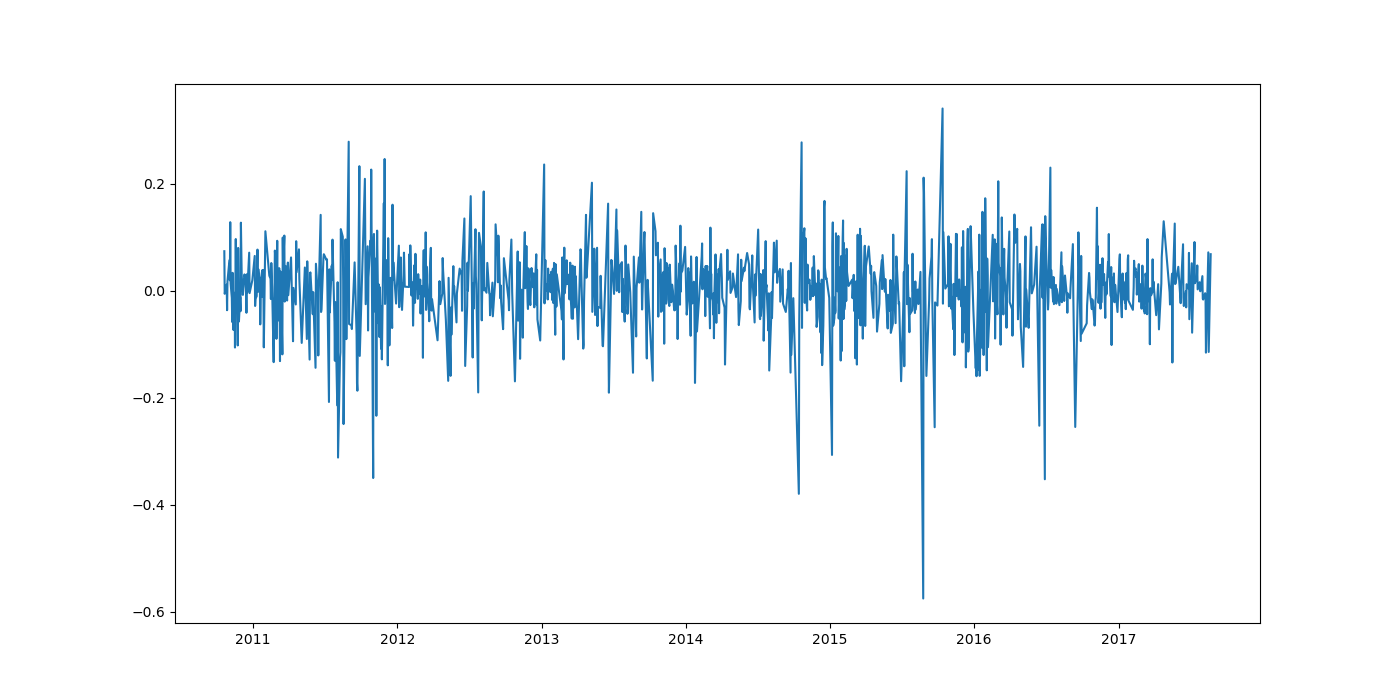
\includegraphics[width=\textwidth]{figures/Ass2/Ass2_Q4_1diff_Close_signal.png}
    \end{minipage}
    \caption{The $1^{st}$ order differencing of "Close price" data.}
    \label{fig:Ass2_Q4_1diff_Close_signal}
\end{figure}

\begin{figure}[H]
    \centering
    \begin{minipage}[b]{1\textwidth}
        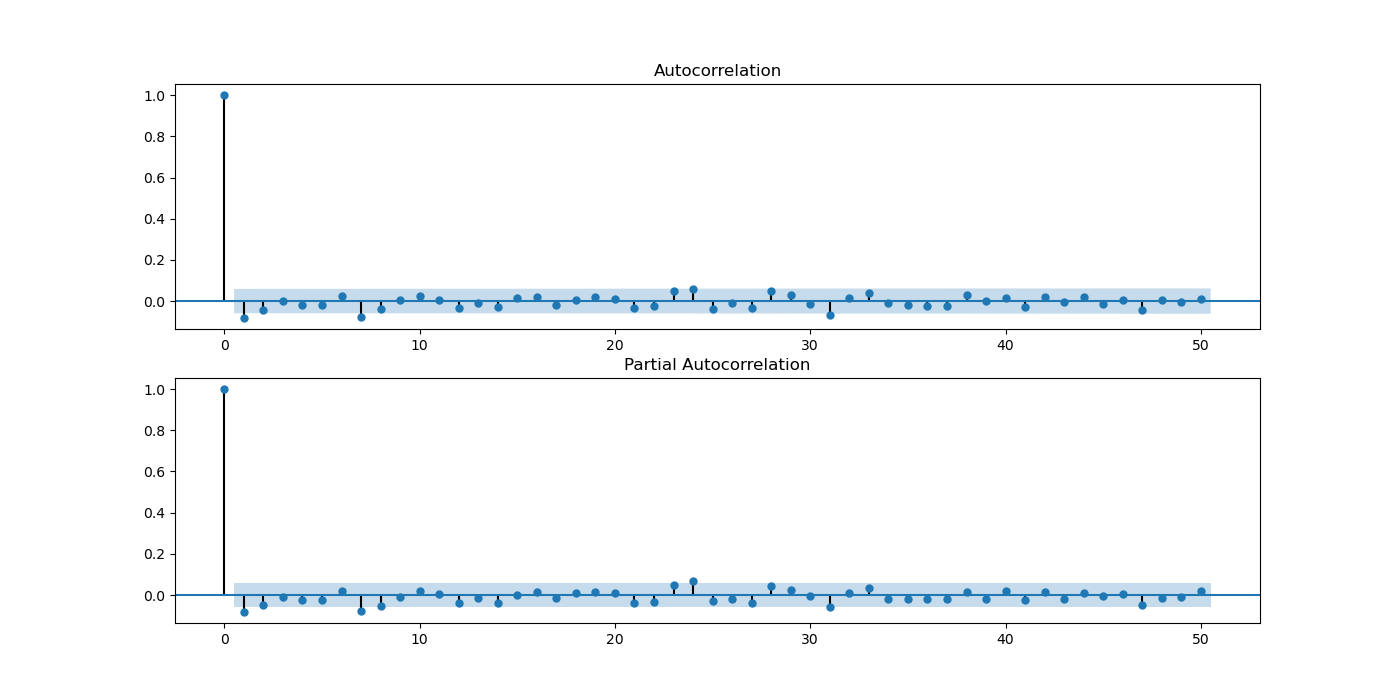
\includegraphics[width=\textwidth]{figures/Ass2/Ass2_Q3_PACF_ACF_1diff.png}
    \end{minipage}
    \caption{A plot of \gls{ACF} and \gls{PACF} on the $1^{st}$ order differencing in "Close price".}
    \label{fig:Ass2_Q4_PACF_ACF_1diff}
\end{figure}

\begin{table}[H]
\centering
\caption{The result of the \gls{ADF} on the $1^{st}$ order differencing variables.}
\label{tab:Ass2_Q4_ADF_results2}
{\tiny
\hspace*{-2cm}\begin{tabular}{lrrrrrrrrrrrr}
\toprule
{} &        Close &           mom &         mom1 &         ROC\_5 &        ROC\_10 &        ROC\_15 &        ROC\_20 &       EMA\_10 &       EMA\_20 &       EMA\_50 &      EMA\_200 &           Oil \\
\midrule
ADF Statistic               &   -25.69 & -12.13 &   -24.15 & -10.63 & -9.74 & -6.99 & -8.059 & -13.44 & -10.72 & -6.82 &    -4.72 & -8.91 \\

p-value                     &     0 &  1.7e-22 &     0 &  4.9e-19 &  8.1e-17 &  7.4e-10 &  1.6e-12 &  3.7e-25 &  3.0e-19 &  1.9e-09 &     7.6e-5 &  1.0e-14 \\
\#Lags Used                  &     1 &  11 &     1 &  9 &  6 &  16 &  5 &  2 &  2 &  5 &     6 &  10 \\
\# Observations Used &  1111 &  1101 &  1111 &  1103 &  1106 &  1096 &  1107 &  1110 &  1110 &  1.107 &  1106 &  1102 \\
Critical Value (1\%)         &    -3.436 & -3.436 & -3.436 &    -3.436 & -3.436 &    -3.436 & -3.436 & -3.436 & -3.436 & -3.436 & -3.436 & -3.436 \\
Critical Value (5\%)         &    -2.864 & -2.864 & -2.864 &    -2.864 & -2.864 &    -2.864 & -2.864 & -2.864 & -2.864 & -2.864 & -2.864 & -2.864 \\
Critical Value (10\%)        &    -2.568 & -2.568 & -2.568 &    -2.568 & -2.568 &    -2.568 & -2.568 & -2.568 & -2.568 & -2.568 & -2.568 & -2.568\\
\bottomrule
\end{tabular}\hspace*{-2cm}
}
\end{table}


\textit{After transforming and making stationary, we needed to find the best-fitted model. Thus we searched on different orders. For the searching area, we used all lags between 1 and 50. Figure \ref{fig:Ass2_Q4_AIC_plot} shows the \gls{AIC} over the different orders. The best order in terms of \gls{AIC} belonged to order 9 (VAR(9) model). We could do the same procedure to find the best order based on other information criteria. The table below shows these results.}

\begin{table}[H]
\centering
\caption{The result of other information criteria.}
\label{tab:Ass2_Q4_criteria}
\begin{tabular}{rlc}
\toprule
\# &  Information Criteria &   Best order \\
\midrule
1 & AIC  &  9 \\
2 & BIC  &  3\\
3 & FPE  &  9\\
4 & HQIC &  5\\
\bottomrule
\end{tabular}

\end{table}


\begin{figure}[H]
    \centering
    \begin{minipage}[b]{1\textwidth}
        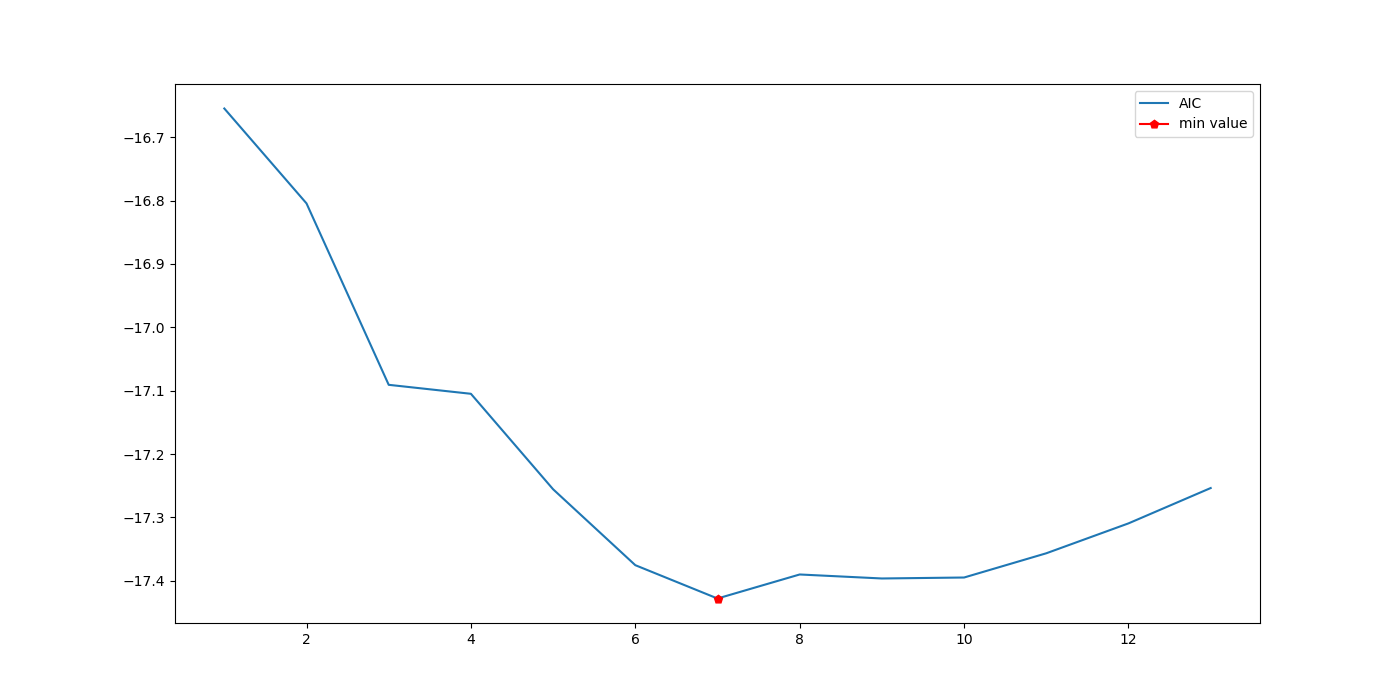
\includegraphics[width=\textwidth]{manuscript/src/figures/Ass2/Ass2_Q4_AIC_plot.png}
    \end{minipage}
    \caption{The \gls{AIC} over the different orders of VAR model.}
    \label{fig:Ass2_Q4_AIC_plot}
\end{figure}

\textit{Figure \ref{fig:Ass2_Q4_residual_plot} indicates the residual of fitted model only for the first variable. As this plot illustrates, the residual signal of model had a Gaussian distribution with zero mean. In addition, the \gls{ACF} plot shows that this signal is a stationary signal.}



\begin{figure}[H]
    \centering
    \begin{minipage}[b]{1\textwidth}
        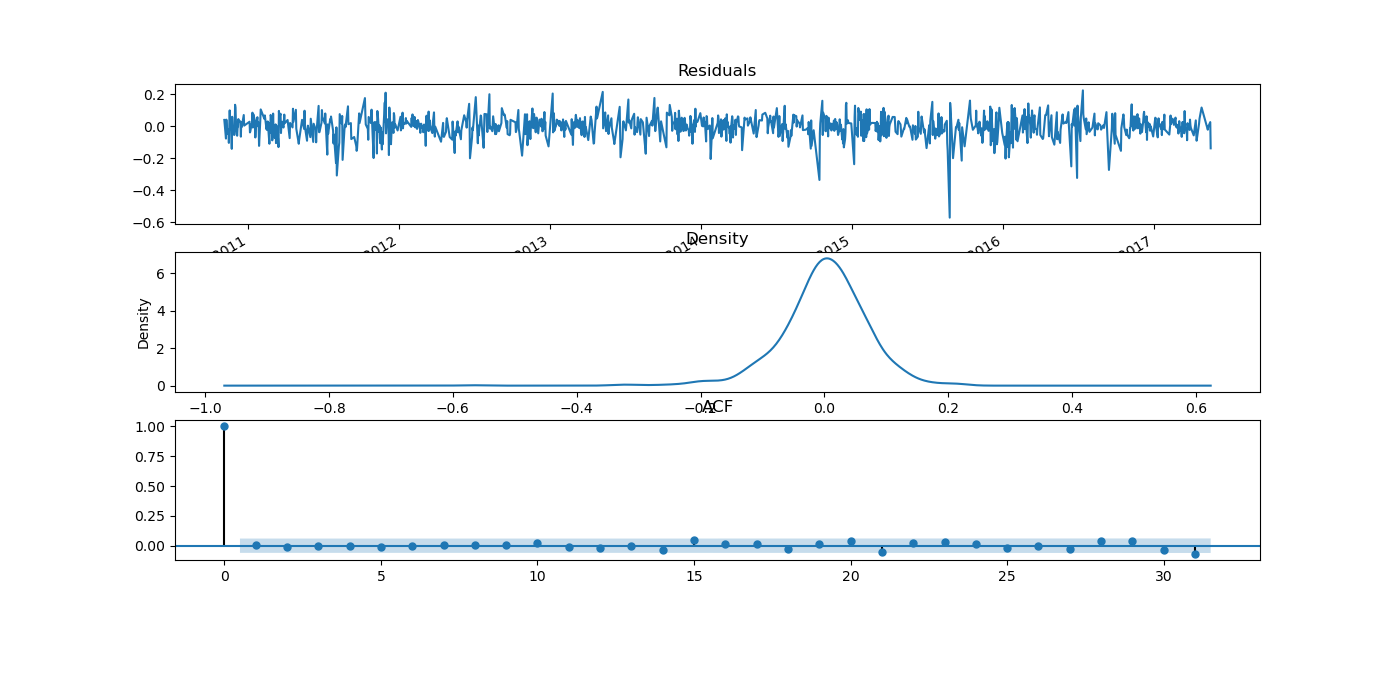
\includegraphics[width=\textwidth]{manuscript/src/figures/Ass2/Ass2_Q4_residual_plot.png}
    \end{minipage}
    \caption{The residual of the fitted model.}
    \label{fig:Ass2_Q4_residual_plot}
\end{figure}


\textit{In addition, we applied Durbin Watson Statistic to estimate their correlation between residuals. This correlation shows whether or not pattern has any leftover pattern in the residuals. As table \ref{tab:Ass2_Q4_DW_results} indicates Durbin Watson results were close to 2. It means there are not correlation between residuals. } 

\begin{table}[H]
\centering
\caption{The result of Durbin Watson test on the dataset.}
\label{tab:Ass2_Q4_DW_results}
\begin{tabular}{rll}
\toprule
\# &  Variable Name &   The result \\
\midrule
1 & Close   &   1.99\\
2 & mom     &   1.98\\
3 & mom1    &   2.0\\
4 & ROC\_5   &   1.99\\
5 & ROC\_10  &   1.99\\
6 & ROC\_15  &   1.97\\
7 & ROC\_20  &   1.97\\
8 & EMA\_10  &   2.0\\
9 & EMA\_20  &   2.0\\
10 & EMA\_50  &   2.0\\
11 & EMA\_200 &        2.0\\
12 & Oil     &    2.0\\
\bottomrule
\end{tabular}




\end{table}




\textit{To forecast, we split data into test and train set like last two parts. After prediction, we reversed differencing and standardization to get the real forecast. Figure \ref{fig:Ass2_Q4_Forecast_vs_Actuals_of_close} demonstrate the output of the fitted model only for "Close price". As can be seen, although the model could predict perfectly at the first, it got flat slope. The RMS error for this model was 339.599.} 


\begin{figure}[H]
    \centering
    \begin{minipage}[b]{1\textwidth}
        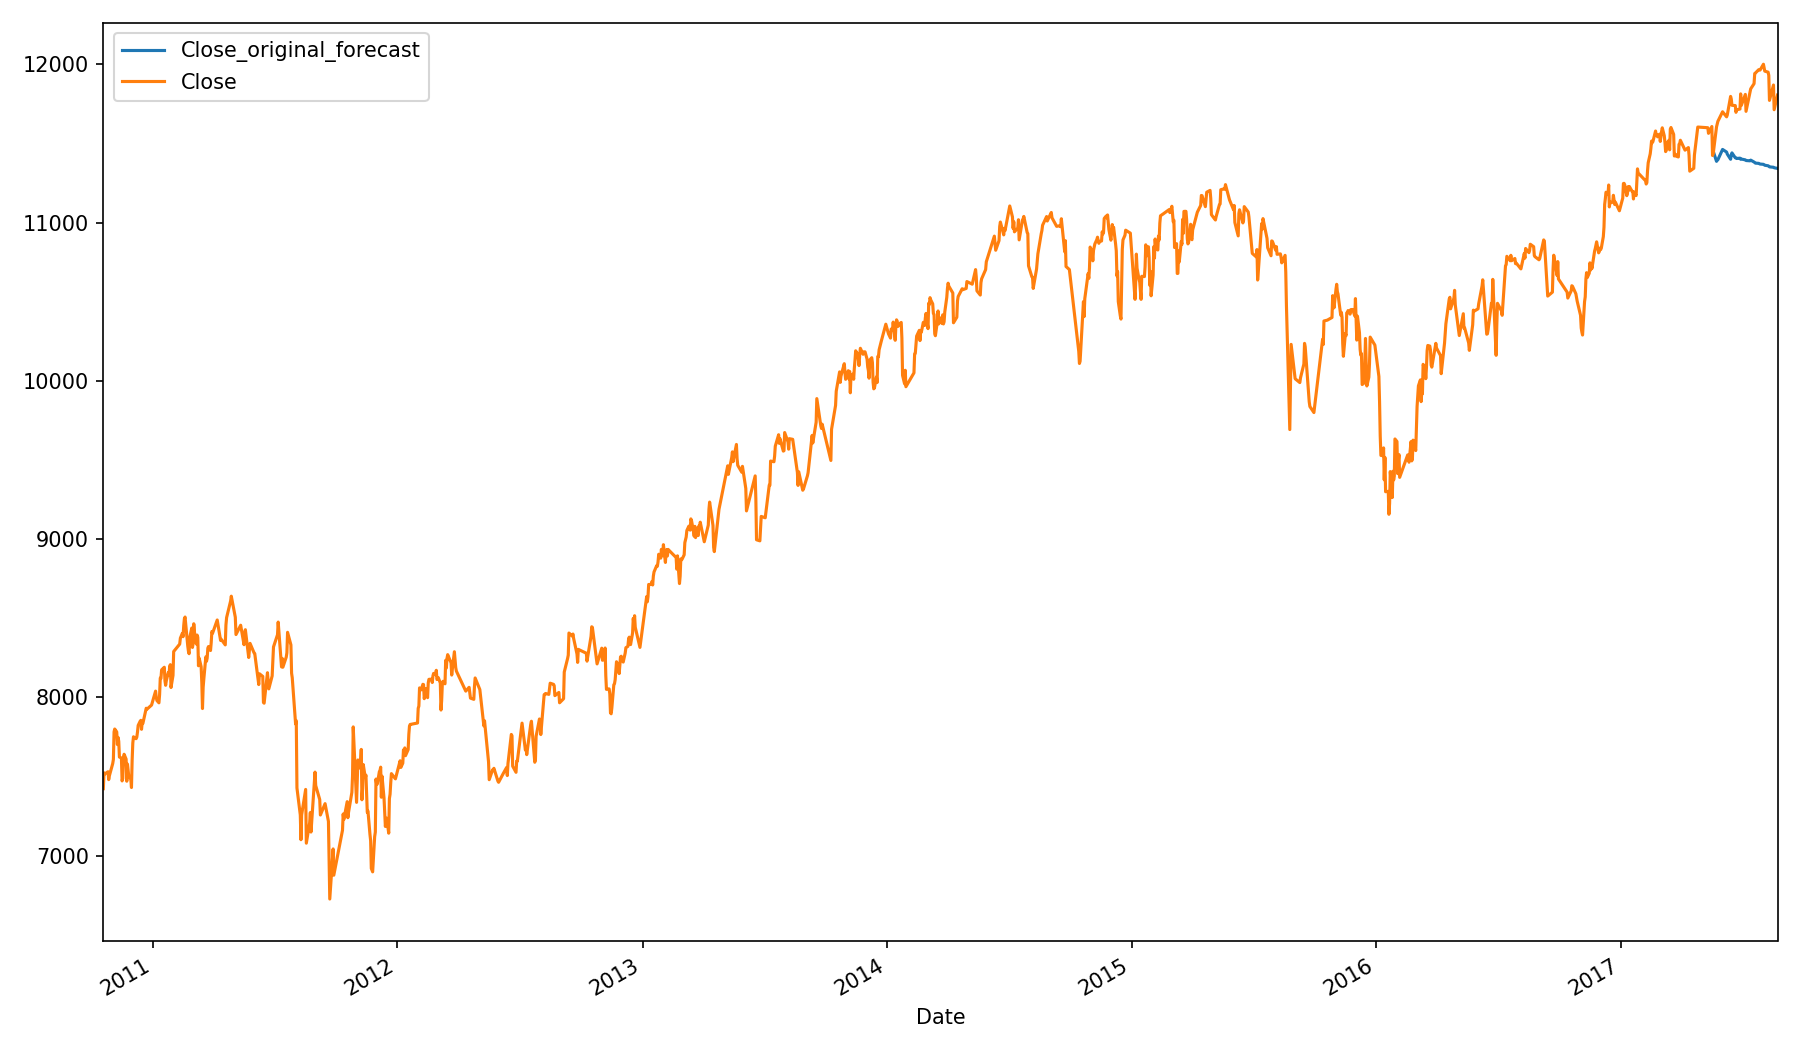
\includegraphics[width=.9\textwidth]{manuscript/src/figures/Ass2/Ass2_Q4_Forecast_vs_Actuals_of_close.png}
    \end{minipage}
    \caption{The prediction and actual data of VAR model.}
    \label{fig:Ass2_Q4_Forecast_vs_Actuals_of_close}
\end{figure}




\textit{For the rolling window approach, we used the same procedure in question 2. Figure \ref{fig:Ass2_Q4_Rolling_Forecast_vs_Actuals_of_close} demonstrate the output of the rolling window model for VAR. As can be seen, the model could follow the the test set better than the previous models. The RMS error decreased to 117.565.}


\begin{figure}[H]
    \centering
    \begin{minipage}[b]{1\textwidth}
        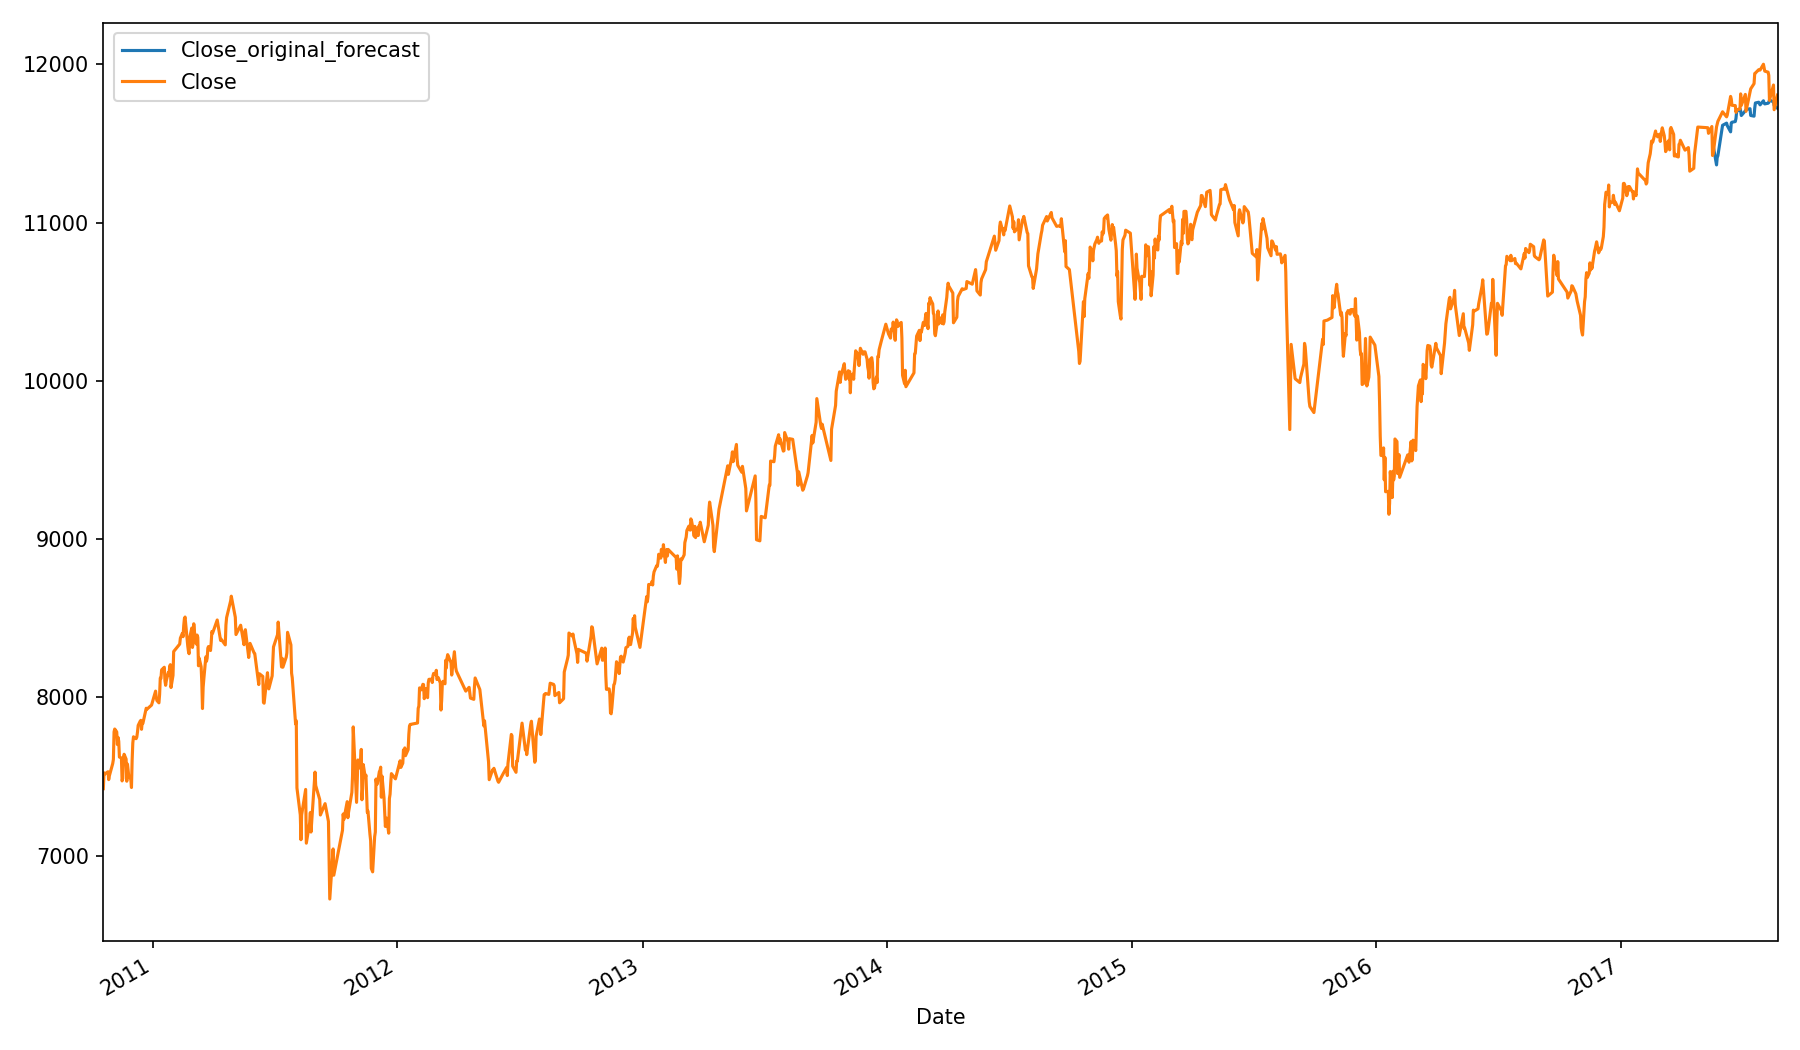
\includegraphics[width=\textwidth]{manuscript/src/figures/Ass2/Ass2_Q4_Rolling_Forecast_vs_Actuals_of_close.png}
    \end{minipage}
    \caption{The prediction and actual data of VAR model.}
    \label{fig:Ass2_Q4_Rolling_Forecast_vs_Actuals_of_close}
\end{figure}